\documentclass[a4paper,12pt]{article} % format du document
\usepackage[utf8x]{inputenc} % encodage des caracteres
\usepackage[francais]{babel} % alinea au debut des sections, sous-sections,...
\usepackage{fullpage} % marges plus classiques
\usepackage{graphicx} % \includegraphics[]{}
\usepackage{float} % gestion des figures
\usepackage{subfig} % gestion des figures
\usepackage{url} % \url{http://}
\usepackage{color} % definition de nouvelles couleurs
\usepackage{amsmath} % tabular
\usepackage{amsfonts} % \mathbb{N}
\usepackage{amssymb} % \mathbb{N}
\usepackage{moreverb}
\usepackage[pdftex,                %
    bookmarks         = true,%     % Signets
    bookmarksnumbered = true,%     % Signets numerotes
    pdfpagemode       = None,%     % Signets/vignettes ferme a l'ouverture
    pdfstartview      = FitH,%     % La page prend toute la largeur
    pdfpagelayout     = SinglePage,% Vue par page
    colorlinks        = false,%     % Liens en couleur
    pdfborder         = {0 0 0}%   % Style de bordure : ici, pas de bordure
    ]{hyperref}%                   % Utilisation de HyperTeX

\hypersetup {
colorlinks=false;
bookmarks=true;
pdftitle={Titre du document}
pdtauthor={Huraux Thomas et Christophe Labedan}
pdfsubject={Sujet du document}
pdfcreator  = {PDFLaTeX}
pdfproducer = {PDFLaTeX}
}
\title{Documentation d\'eveloppeur}
\author{Thomas Huraux et Christophe Labedan}
\date{}
\begin{document}
\maketitle

\section*{Interface}
Afin de b\'en\'eficier des services offert par le container de jeux de NoBrainer il suffit d'impl\'ementer l'interface \emph{fr.uhp.nobrain.games.GameState}.

\begin{figure}[htbp]
\centering
 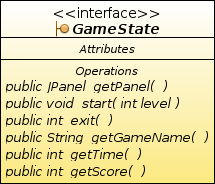
\includegraphics[width=.25\linewidth]{GameStateInterfaceDiagram.png}
\end{figure}

\section*{Configuration}
Chaque jeu doit \^etre contenu dans une archive Jar. Pour ajouter un jeu, il suffit alors d'ajouter une ligne dans le fichier \emph{conf.txt} avec le chemin vers le .jar ainsi que le nom de l'interface. Les jeux seront charg\'es dynamiquement lors du d\'emarrage d'une nouvelle partie. L'enchainement des diff\'erents jeux se fera en correspondance avec l'ordre dans le fichier de configuration.

Exemple d'un fichier de configuration :
\begin{center}
 \begin{verbatim}
------------------------------ conf.txt ------------
src/main/resources/games/GameLetter.jar GameLetter
src/main/resources/games/GameNumber.jar GameNumber
----------------------------------------------------
 \end{verbatim}
\end{center}

\section*{Affichage}
Pas besoin de g\'erer l'affichage du score ni du temps restant. Le container viendra chercher \`a intervalle r\'egulier le score \`a l'aide de la m\'ethode \emph{getScore} d\'eclar\'ee dans l'interface. L'ensemble de l'affichage devra \^etre contenu dans un JPanel que le container pourra r\'ecup\'erer \`a tout moment avec \emph{getPanel}. La fonction \emph{getTime} permettra au container de de g\'erer le temps de jeu tout en affichant en temps r\'eel le temps restant.

\end{document}